% ex: ts=2 sw=2 sts=2 et filetype=tex
% SPDX-License-Identifier: CC-BY-SA-4.0

\documentclass[12pt,addpoints]{exam}

\usepackage[utf8]{inputenc}
\usepackage[T1]{fontenc}
%\usepackage[spanish]{babel}
\usepackage[letterpaper]{geometry}

\pagestyle{headandfoot}
\headrule
\header{Física II}{Examen 2º Parcial}{CBTIS 246}
\footer{}{Página \thepage\ de \numpages}{}

\pointpoints{punto}{puntos}
\renewcommand{\solutiontitle}{\textbf{Solución: }}


\newcommand{\makenonemptybox}[2]{%
  \par\nobreak\vspace{\ht\strutbox}\noindent
  \fbox{%
    \parbox[c][\dimexpr#1-2\fboxsep][t]{\dimexpr\linewidth-2\fboxsep}{
      \hrule width \hsize height 0pt
      #2
    }%
  }%
  \par\vspace{\ht\strutbox}
}
\makeatother

%\printanswers

\begin{document}
%\begin{center}
%\fbox{\fbox{\parbox{5.5in}{\centering
%Lee con atención cada pregunta y responde en
%el espacio ubicado en la parte izquierda.
%}}}
%\end{center}
%
%\vspace{5mm}

Nombre:\enspace\hrulefill

\vspace{5mm}

Grupo:\enspace\hrulefill
\enspace{}Grado:\enspace\hrulefill
\enspace{}Fecha:\enspace\hrulefill

\begin{questions}

% ex: ts=2 sw=2 sts=2 et filetype=tex
% SPDX-License-Identifier: CC-BY-SA-4.0

\question $c^2 + 5c - 24$


% ex: ts=2 sw=2 sts=2 et filetype=tex
% SPDX-License-Identifier: CC-BY-SA-4.0

\question ¿Qué es rotación, traslación y percepción espacial?:

% ex: ts=2 sw=2 sts=2 et filetype=tex
% SPDX-License-Identifier: CC-BY-SA-4.0

\question 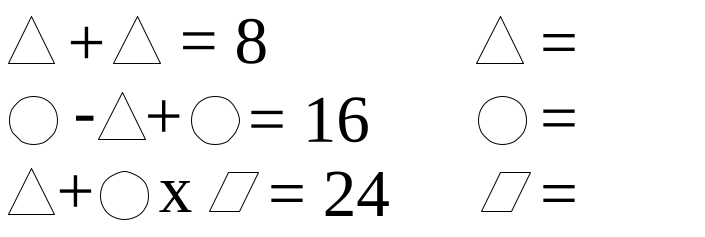
\includegraphics[scale=0.5]{p/i01.png}


% ex: ts=2 sw=2 sts=2 et filetype=tex
% SPDX-License-Identifier: CC-BY-SA-4.0

\question 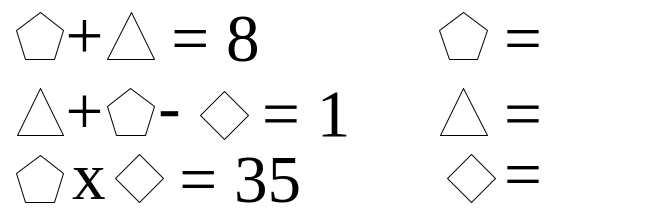
\includegraphics[scale=0.5]{p/i02.png}


% ex: ts=2 sw=2 sts=2 et filetype=tex
% SPDX-License-Identifier: CC-BY-SA-4.0

\question Escribe los siguientes números en notación cientifica:

  \begin{parts}
    \part $45,000 = $
    \part $0.045 = $
    \part $8,900 = $
  \end{parts}

% ex: ts=2 sw=2 sts=2 et filetype=tex
% SPDX-License-Identifier: CC-BY-SA-4.0

\question Un resorte de $10 cm$ de longitud recibe una magnitud de fuerza
          que lo restira hasta medir $15 cm$ ¿Cuál es la magnitud de la
          tensión unitaria o deformación lineal?

\makenonemptybox{1.6in}{Datos: \hspace{1cm} Formula: \hspace{1cm}
                      Despeje: \hspace{1cm} Sustitución y Resultado}

% ex: ts=2 sw=2 sts=2 et filetype=tex
% SPDX-License-Identifier: CC-BY-SA-4.0

\question Encontrar los divisores de 30:

  \begin{solutionorlines}[1cm]
    Div.(30):\{1,3,5,6,10,15,30\}
  \end{solutionorlines}

% ex: ts=2 sw=2 sts=2 et filetype=tex
% SPDX-License-Identifier: CC-BY-SA-4.0

\question Un resorte, cuyo módulo de elasticidad es de $50$\textbf{N/m}
          recibe un esfuerzo con una magnitud de $18$\textbf{N} ¿Cuál es su
          deformación?

\makenonemptybox{1.6in}{Datos: \hspace{1cm} Formula: \hspace{1cm}
                      Despeje: \hspace{1cm} Sustitución y Resultado}


\end{questions}

\end{document}
